\section{Classification de caract\'eristiques locales}

Dans la suite du TP, nous avons choisi de traiter le probl\`eme \textit{Visages} de la base d'images Essex. L'objectif g\'en\'eral est d'isoler les pixels de la peau du reste de l'image, afin de localiser pr\'ecis\'ement le visage sur l'image \`a partir d'une classification de caract\'eristiques locales.

\subsection{Classification bayésienne des pixels}

%TODO: Reducri cantidad de texto, dejar lo verdaderamente importante de esta seccion

La classification bay\'esienne des pixels consiste \`a attribuer \`a chaque pixel de l'image une classe en fonction d'un vecteur d'observation construit \`a partir de caract\'eristiques locales, typiquement les composantes de couleur ou d'autres descripteurs calcul\'es autour du pixel. Dans le cadre de ce TP, l'id\'ee est de mod\'eliser probabilistiquement chaque classe \`a partir d'exemples annot\'es, puis de d\'ecider pour chaque pixel la classe la plus probable au sens bay\'esien.

Conform\'ement \`a la section 3.1 du sujet, on commence par visualiser les composantes pertinentes avec le script \texttt{Display\_Components.py}, puis on s\'electionne des exemples d'apprentissage pour apprendre un mod\`ele avec \texttt{Bayes\_Model\_Training.py}. L'apprentissage est supervis\'e : l'utilisateur fournit, \`a l'aide de la souris et du clavier, des r\'egions d'exemples appartenant \`a la classe positive et \`a la classe n\'egative. Le mod\`ele estim\'e permet ensuite de classer l'ensemble des pixels de l'image selon la probabilit\'e associ\'ee \`a chaque classe.

Dans notre probl\`eme \textit{Visages}, cette approche revient \`a distinguer principalement les pixels de peau des pixels de non-peau. La classe positive correspond donc aux zones du visage que l'on souhaite extraire, tandis que la classe n\'egative regroupe l'arri\`ere-plan, les cheveux, les v\^etements et les autres parties de l'image. L'objectif est d'obtenir une segmentation suffisamment pr\'ecise pour localiser le visage de mani\`ere fiable.

\subsubsection{Analyse des couleurs}

Afin d'\'evaluer la s\'eparabilit\'e visuelle entre la peau et le non-peau avant 
l'apprentissage, nous avons ex\'ecut\'e le script \texttt{Display\_Components.py} 
sur l'image \texttt{img/Essex\_Faces/94/asamma.19.jpg}, issue du jeu de donn\'ees 
des visages. Les sorties ont \'et\'e sauvegard\'ees dans 
\texttt{outputs/components/asamma.19/rgb}, 
\texttt{outputs/components/asamma.19/hsv} et 
\texttt{outputs/components/asamma.19/ycrcb} (voir Figure \ref{fig:face_components_spaces}). 
Les fichiers \texttt{original.png} pr\'esents dans chacun de ces r\'epertoires correspondent \`a la m\^eme image source, tandis que les figures de synth\`ese permettent de comparer les d\'ecompositions dans les trois espaces colorim\'etriques.

\begin{figure*}[htbp]
\centering
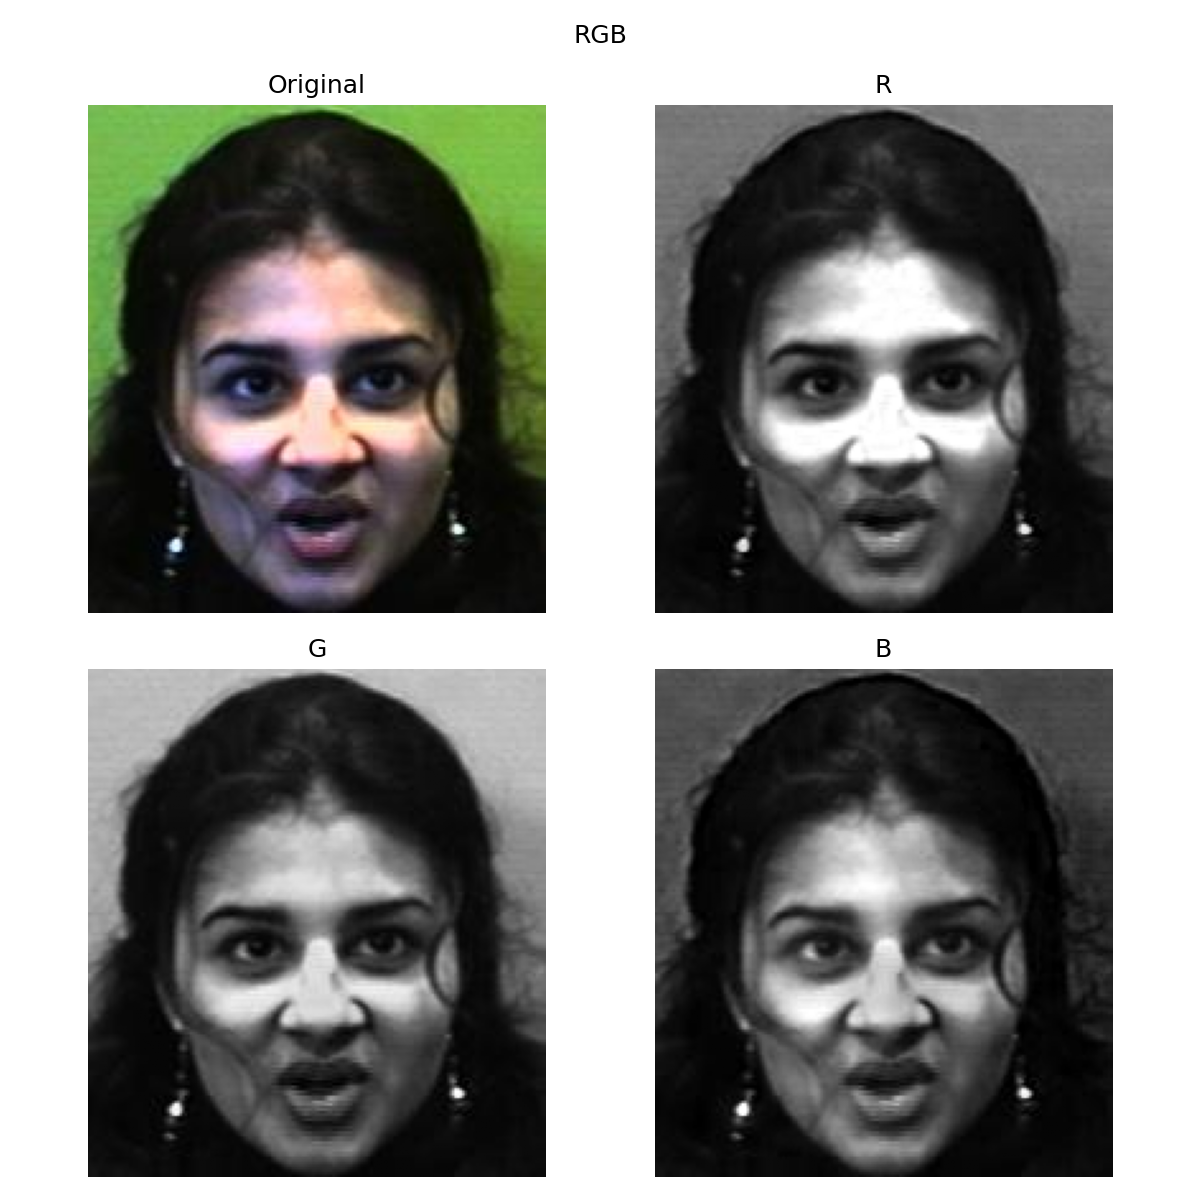
\includegraphics[width=0.32\textwidth]{../../outputs/components/asamma.19/rgb/figure.png}\hfill
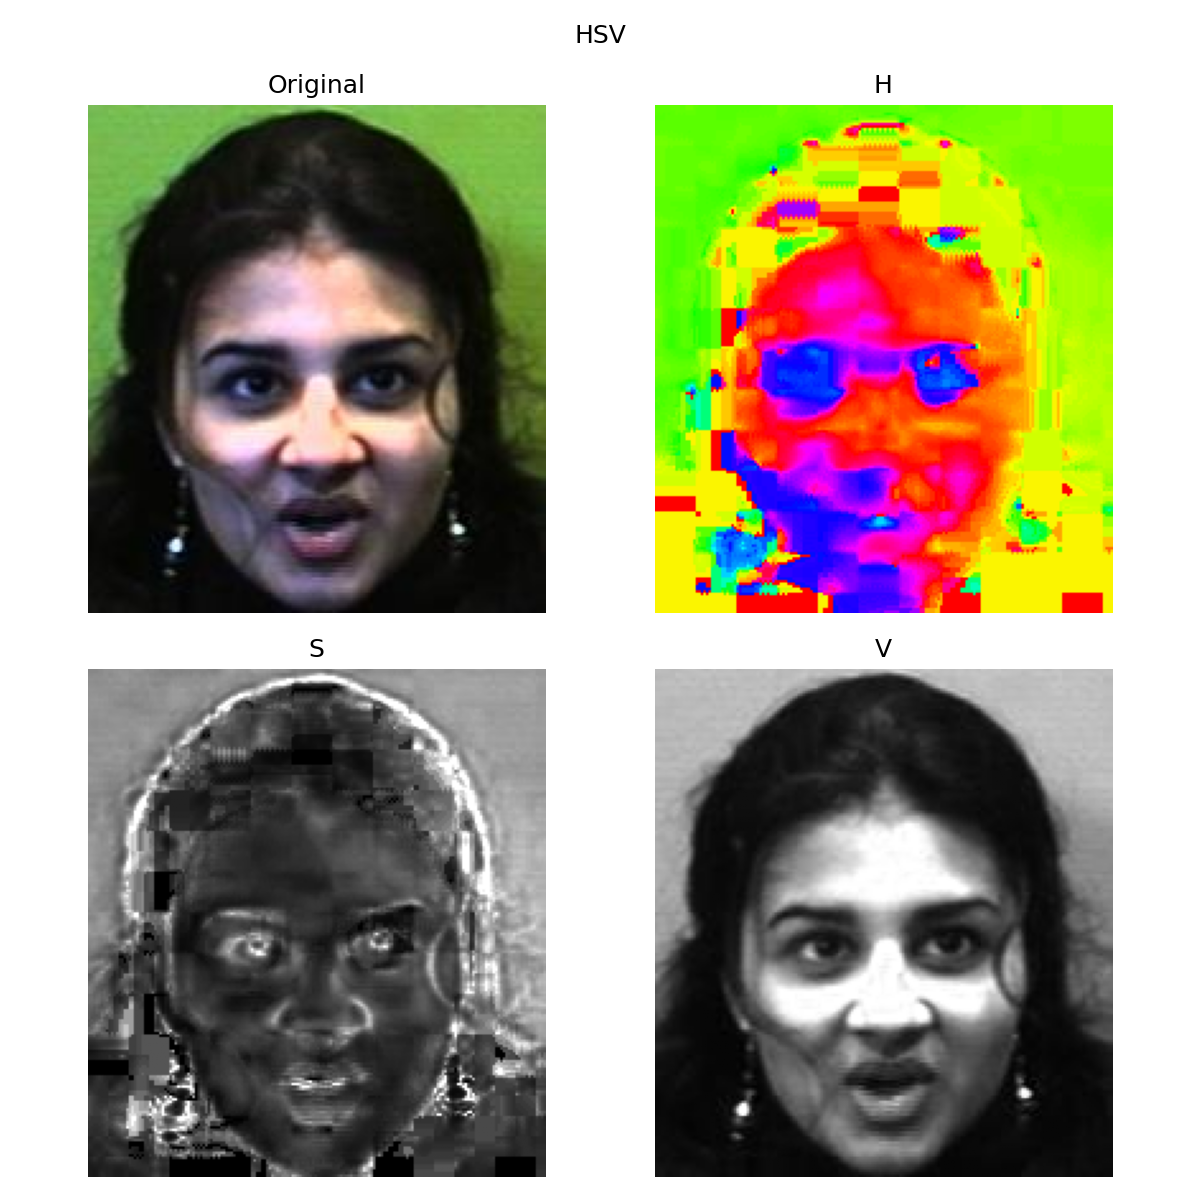
\includegraphics[width=0.32\textwidth]{../../outputs/components/asamma.19/hsv/figure.png}\hfill
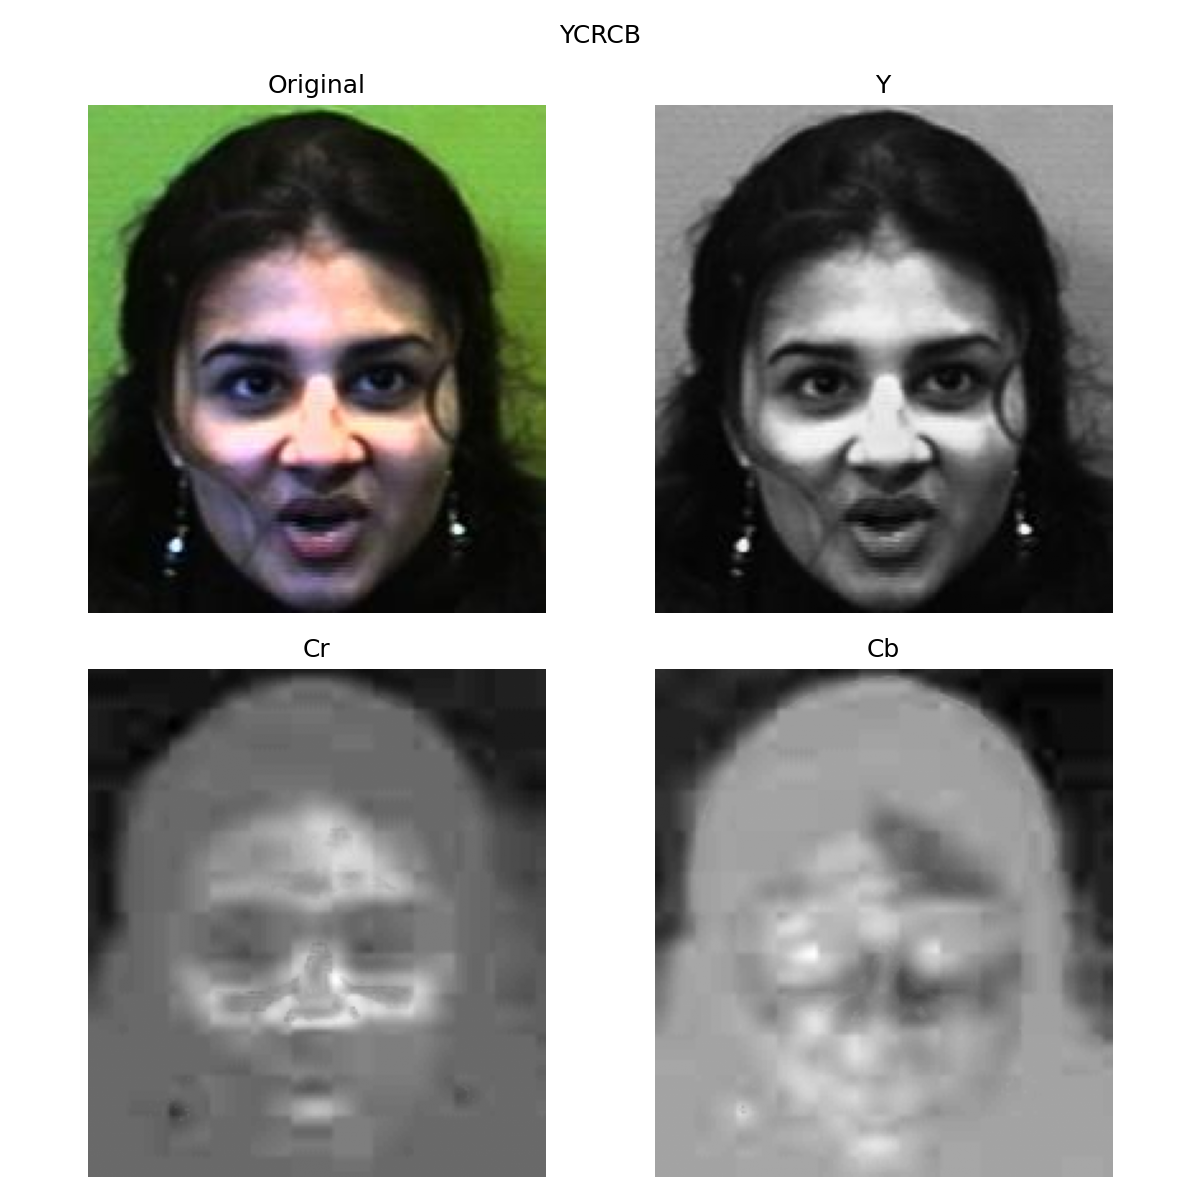
\includegraphics[width=0.32\textwidth]{../../outputs/components/asamma.19/ycrcb/figure.png}
\caption{D\'ecompositions RGB, HSV et YCrCb de l'image \texttt{asamma.19.jpg}, g\'en\'er\'ees avec \texttt{Display\_Components.py}. Chaque figure contient l'image originale ainsi que les trois composantes de l'espace consid\'er\'e.}
\label{fig:face_components_spaces}
\end{figure*}

L'espace RGB fournit une lecture directe des intensit\'es rouge, verte et bleue, mais il m\'elange l'information de chrominance et l'information d'illumination. Sur cette image, le fond vert est relativement bien distingu\'e dans le canal \(G\), et la peau ressort davantage dans le canal \(R\). N\'eanmoins, les variations d'\'eclairage sur le front, le nez et les joues restent fortement pr\'esentes dans les trois canaux, ce qui risque de rendre le mod\`ele moins stable d'une image \`a l'autre.

L'espace HSV s\'epare partiellement la couleur de la luminance via les composantes \(H\), \(S\) et \(V\). La composante \(V\) conserve la structure g\'en\'erale du visage, mais la composante \(H\) appara\^it ici plus instable et bruit\'ee, notamment dans les zones de faible saturation ou pr\`es des transitions abruptes. La composante \(S\) met en \'evidence certaines diff\'erences de peau et de fond, mais elle reste sensible aux reflets, aux ombres et aux zones sombres comme les cheveux.

L'espace YCrCb est le plus prometteur pour ce probl\`eme. La composante \(Y\) capture la luminance et donc la structure g\'en\'erale de la sc\`ene, tandis que \(Cr\) et \(Cb\) isolent mieux l'information chromatique li\'ee \`a la peau. Dans les r\'esultats obtenus, le visage reste relativement coh\'erent dans les composantes \(Cr\) et \(Cb\), alors que l'arri\`ere-plan et les cheveux se distinguent plus nettement. Cette d\'ecorr\'elation entre luminance et chrominance est favorable \`a l'apprentissage d'un mod\`ele bay\'esien plus robuste pour la d\'etection de la peau.

En cons\'equence, YCrCb constitue le meilleur point de d\'epart pour construire un bon mod\`ele de d\'etection dans notre cas. Il existe cependant des opportunit\'es claires pour enrichir l'espace d'observation avec des caract\'eristiques locales personnalis\'ees. Une premi\`ere piste consiste \`a combiner \(Cb\) et \(Cr\) avec une mesure de structure locale, par exemple le gradient de \(Y\), afin d'introduire \`a la fois l'information de couleur de peau et l'information de contour. Une autre piste est d'utiliser des moyennes locales, des \'ecarts-types sur fen\^etre, ou des descripteurs de texture locale pour mieux distinguer la peau des cheveux, des ombres et de l'arri\`ere-plan. Cette id\'ee est coh\'erente avec l'extension \texttt{cbcr\_grad} d\'ej\`a pr\'esente dans le code, qui combine \(Cb\), \(Cr\) et \(|\nabla Y|\) pour enrichir la repr\'esentation locale des pixels.

\subsubsection{Propres caractéristiques locales}

Pour aller au-del\`a de l'utilisation des seules composantes de couleur,
 nous avons ajout\'e une caract\'eristique locale de type 
 \textit{gradient et chrominance}, not\'ee \texttt{cbcr\_grad}, 
 et visualis\'ee avec une extension du script 
 \texttt{Display\_Components.py}. Cette repr\'esentation combine 
 les composantes \(Cb\) et \(Cr\), qui conservent l'information de 
 chrominance li\'ee \`a la peau, avec la norme du gradient 
 \(|\nabla Y|\), calcul\'ee sur la luminance. Les sorties 
 correspondantes ont \'et\'e enregistr\'ees dans 
 \texttt{outputs/components/asamma.19/cbcr\_grad} (voir Figure \ref{fig:face_cbcr_grad}).

\begin{figure}[htbp]
\centering
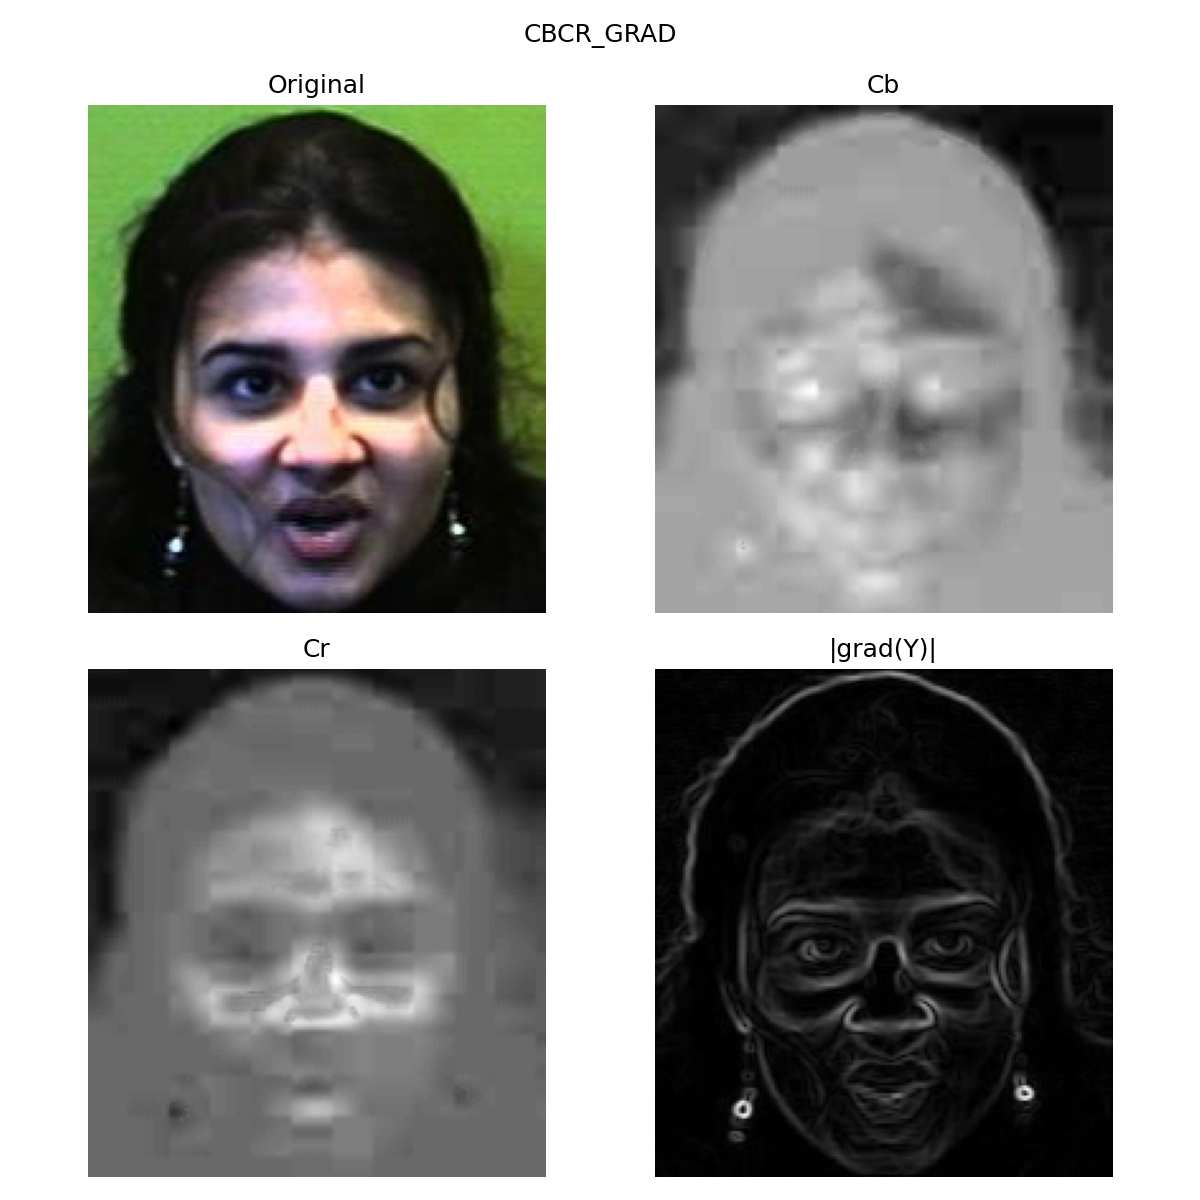
\includegraphics[width=0.95\columnwidth]{../../outputs/components/asamma.19/cbcr_grad/figure.png}
\caption{Visualisation de la caract\'eristique locale \texttt{cbcr\_grad} sur l'image \texttt{asamma.19.jpg} : image originale, \(Cb\), \(Cr\) et \(|\nabla Y|\).}
\label{fig:face_cbcr_grad}
\end{figure}

Les composantes \(Cb\) et \(Cr\) gardent une bonne coh\'erence sur les zones de peau, comme dans l'espace YCrCb, mais l'ajout de \(|\nabla Y|\) fait appara\^itre plus nettement les contours et transitions locales significatives : bord du visage, yeux, bouche, fronti\`eres entre la peau et les cheveux, ainsi qu'entre le visage et l'arri\`ere-plan. Par rapport \`a YCrCb seul, cette combinaison introduit donc une information de structure locale sans quitter une repr\'esentation compacte \`a trois dimensions.

Cette caract\'eristique est plus favorable \`a un mod\`ele bay\'esien de d\'etection peau / non-peau, car elle aide \`a mieux distinguer les r\'egions ambigu\"es o\`u la couleur seule ne suffit pas, en particulier sur les fronti\`eres et dans les zones partiellement ombr\'ees. Sa limite est que le gradient r\'eagit aussi aux ombres, \`a certaines textures et aux accessoires. En pratique, cela signifie que les exemples n\'egatifs utilis\'es pendant l'apprentissage doivent couvrir non seulement le fond, mais aussi les cheveux, les yeux et les zones sombres du visage, afin d'\'eviter qu'un contour marqu\'e soit confondu avec une zone de peau.
